% Guided Soft Actor-Critic for Go2-W — theory & implementation slides.
% Mirrors flashsac_go2w_fable/gsac/ (config.py, network.py, update.py, agent.py)
% and docs/guided_sac_design.md (rev. 3). No experimental results by design.
\documentclass[aspectratio=169]{beamer}
\usetheme{metropolis}

\usepackage{amsmath,amssymb}
\usepackage{booktabs}
\usepackage{tikz}
\usetikzlibrary{positioning,arrows.meta,fit,backgrounds,calc,shapes.geometric,decorations.pathreplacing}

\definecolor{cStudent}{HTML}{1B7F79}
\definecolor{cGuide}{HTML}{B8552B}
\definecolor{cCritic}{HTML}{3B5B92}
\definecolor{cEnv}{HTML}{4A4A4A}
\definecolor{cDrop}{HTML}{9B9B9B}
\definecolor{cAccent}{HTML}{8E44AD}

\tikzset{
  blk/.style={rounded corners=2pt, draw, thick, align=center,
              inner sep=4pt, font=\scriptsize},
  student/.style={blk, draw=cStudent, fill=cStudent!8, text=cStudent!60!black},
  guide/.style={blk, draw=cGuide, fill=cGuide!8, text=cGuide!60!black},
  critic/.style={blk, draw=cCritic, fill=cCritic!8, text=cCritic!60!black},
  envb/.style={blk, draw=cEnv, fill=cEnv!6, text=cEnv},
  dropb/.style={blk, draw=cDrop, fill=cDrop!8, text=cDrop!70!black, dashed},
  ar/.style={-{Stealth[length=4pt]}, thick},
  arg/.style={-{Stealth[length=4pt]}, thick, cGuide},
  ars/.style={-{Stealth[length=4pt]}, thick, cStudent},
  arc/.style={-{Stealth[length=4pt]}, thick, cCritic},
  lbl/.style={font=\tiny, inner sep=1.5pt},
}

\newcommand{\ot}{o_t}
\newcommand{\st}{\tilde{s}_t}
\newcommand{\pf}{\pi_f}
\newcommand{\pg}{\pi_g}

\title{Guided Soft Actor--Critic}
\subtitle{Blind Go2-W Locomotion --- Theory and Implementation}
\author{Tamer Bora İkizoğlu}
\institute{Istanbul Technical University}
\date{}

\begin{document}

\maketitle

\begin{frame}{Outline}
  \tableofcontents
\end{frame}

% =====================================================================
\section{The problem}

\begin{frame}{Blind locomotion is a POMDP}
  \textbf{In simulation} we can read anything: body linear velocity, a height scan of
  the terrain, contact forces, friction, every randomized dynamics parameter.

  \textbf{On the real robot} almost none of that exists. The deployed policy sees only
  proprioception: joint encoders, IMU, its own previous action.

  \vspace{0.6em}
  \begin{alertblock}{The asymmetry}
    Training-time information $\gg$ deployment-time information. A policy trained on
    what it \emph{cannot} have at deployment is useless; a policy that ignores what the
    simulator knows is wasteful.
  \end{alertblock}

  \vspace{0.4em}
  Guided SAC is one answer: let a \emph{privileged} network help train a \emph{blind}
  network that is the only thing shipped.
\end{frame}

\begin{frame}{Two observation channels}
  \begin{center}
  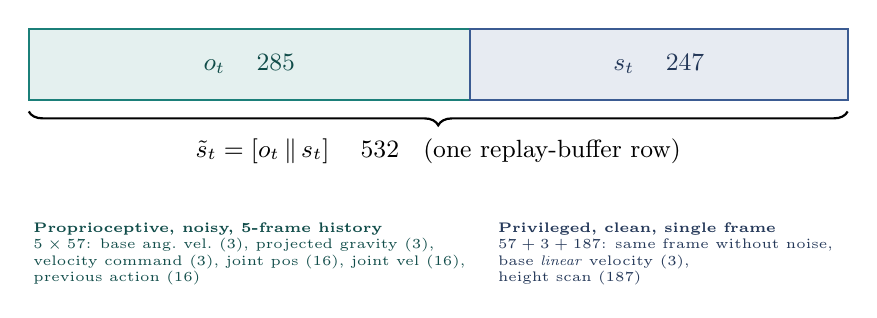
\begin{tikzpicture}[scale=1]
    \draw[fill=cStudent!12, draw=cStudent, thick] (0,0) rectangle (5.6,0.9);
    \node[font=\small, text=cStudent!60!black] at (2.8,0.45) {$\ot$ \;\; 285};
    \draw[fill=cCritic!12, draw=cCritic, thick] (5.6,0) rectangle (10.4,0.9);
    \node[font=\small, text=cCritic!60!black] at (8.0,0.45) {$s_t$ \;\; 247};
    \draw[decorate, decoration={brace, amplitude=5pt, mirror}, thick]
      (0,-0.15) -- (10.4,-0.15) node[midway, below=6pt, font=\small] {$\st = [\ot \,\|\, s_t]$ \;\; 532 \; (one replay-buffer row)};

    \node[lbl, align=left, anchor=north west, text=cStudent!60!black] at (0,-1.5)
      {\textbf{Proprioceptive, noisy, 5-frame history}\\
       $5\times 57$: base ang.\ vel.\ (3), projected gravity (3),\\
       velocity command (3), joint pos (16), joint vel (16),\\
       previous action (16)};
    \node[lbl, align=left, anchor=north west, text=cCritic!60!black] at (5.9,-1.5)
      {\textbf{Privileged, clean, single frame}\\
       $57 + 3 + 187$: same frame without noise,\\
       base \emph{linear} velocity (3),\\
       height scan (187)};
  \end{tikzpicture}
  \end{center}
  \vspace{0.2em}
  {\footnotesize Action space: $16$ dims $=$ 12 leg position targets $+$ 4 wheel velocity
  targets, $\tanh$-squashed and scaled by per-dimension bounds (legs $5.0$, wheels $10.0$).}
\end{frame}

% =====================================================================
\section{Guided SAC: the idea}

\begin{frame}{Origin, and what we changed}
  Haklıdır \& Temeltaş (2021) and Çerçi \& Temeltaş (2024) train \textbf{two actors}:
  a \emph{guiding actor} that sees clean state, and a \emph{control actor} that sees
  degraded state and is pulled toward the guide's actions.

  \vspace{0.5em}
  \begin{center}
  \scriptsize
  \begin{tabular}{lll}
    \toprule
     & \textbf{Çerçi (2024)} & \textbf{This project} \\
    \midrule
    Why the control actor is handicapped & adversarial perturbation & \emph{genuine} partial observability \\
    Guiding actor sees & clean state $s_t$ & privileged $\st$ (height scan, lin.\ vel.) \\
    Control actor sees & perturbed $s^p_t$ & proprioception $\ot$ + history \\
    Shapes & identical & \textbf{different} (285 vs 532) \\
    Agents & $k = 3,5,7$ & $k = 1$ (single agent) \\
    \bottomrule
  \end{tabular}
  \end{center}

  \vspace{0.4em}
  {\footnotesize Two consequences: the paper's $s^p_t \!\to\! \ot$ mapping is \emph{not}
  cosmetic (different dimensionality), and every multi-agent construction collapses at
  $k=1$ --- it must be re-derived, not copied.}
\end{frame}

\begin{frame}{Guided SAC is three mechanisms, not one}
  \begin{center}
  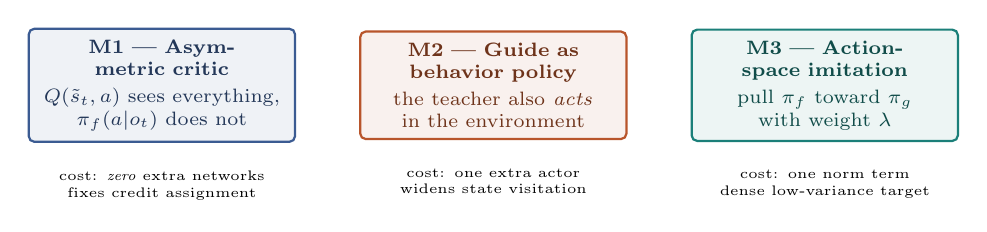
\begin{tikzpicture}[node distance=3mm]
    \node[critic, text width=3.1cm] (m1)
      {\textbf{M1 — Asymmetric critic}\\[2pt] $Q(\st,a)$ sees everything,\\ $\pf(a|\ot)$ does not};
    \node[guide, text width=3.1cm, right=8mm of m1] (m2)
      {\textbf{M2 — Guide as behavior policy}\\[2pt] the teacher also \emph{acts}\\ in the environment};
    \node[student, text width=3.1cm, right=8mm of m2] (m3)
      {\textbf{M3 — Action-space imitation}\\[2pt] pull $\pf$ toward $\pg$\\ with weight $\lambda$};
    \node[lbl, below=3mm of m1, text width=3.1cm, align=center] {cost: \emph{zero} extra networks\\ fixes credit assignment};
    \node[lbl, below=3mm of m2, text width=3.1cm, align=center] {cost: one extra actor\\ widens state visitation};
    \node[lbl, below=3mm of m3, text width=3.1cm, align=center] {cost: one norm term\\ dense low-variance target};
  \end{tikzpicture}
  \end{center}
  \vspace{0.8em}
  The literature ships these \textbf{bundled}. Separating them matters: M1 is free and not
  specific to Guided SAC, while M2 is the expensive one. Our design keeps M1, keeps M3 in
  softened form, and uses only a \emph{small} amount of M2 --- for a different reason than
  the original (next slides).
\end{frame}

% =====================================================================
\section{Architecture}

\begin{frame}{Three networks}
  \begin{center}
  \scalebox{0.95}{%
  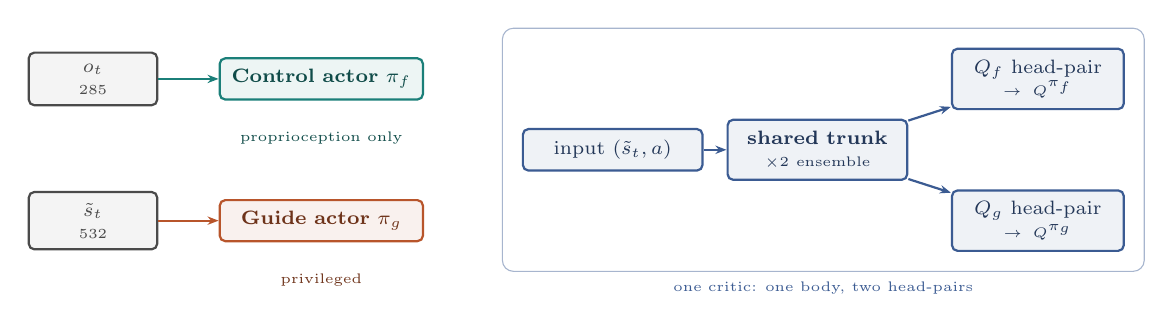
\begin{tikzpicture}[x=1cm, y=1cm]
    % --- actors ---
    \node[envb,    text width=1.35cm] (o)  at (0,1.3)    {$\ot$\\ \tiny 285};
    \node[student, text width=2.3cm]  (pf) at (2.9,1.3)  {\textbf{Control actor} $\pf$};
    \node[envb,    text width=1.35cm] (sv) at (0,-0.5)   {$\st$\\ \tiny 532};
    \node[guide,   text width=2.3cm]  (pg) at (2.9,-0.5) {\textbf{Guide actor} $\pg$};
    \draw[ars] (o)  -- (pf);
    \draw[arg] (sv) -- (pg);
    \node[lbl, text=cStudent!60!black] at (2.9,0.55) {proprioception only};
    \node[lbl, text=cGuide!60!black]   at (2.9,-1.25) {privileged};

    % --- critic ---
    \node[critic, text width=2.0cm] (in) at (6.6,0.4)  {input $(\st, a)$};
    \node[critic, text width=2.0cm] (tr) at (9.2,0.4)  {\textbf{shared trunk}\\ \tiny $\times 2$ ensemble};
    \node[critic, text width=1.9cm] (qf) at (12.0,1.3) {$Q_f$ head-pair\\ \tiny $\to Q^{\pf}$};
    \node[critic, text width=1.9cm] (qg) at (12.0,-0.5){$Q_g$ head-pair\\ \tiny $\to Q^{\pg}$};
    \draw[arc] (in) -- (tr);
    \draw[arc] (tr) -- (qf);
    \draw[arc] (tr) -- (qg);
    \begin{scope}[on background layer]
      \node[fit=(in)(tr)(qf)(qg), draw=cCritic!45, rounded corners, inner sep=7pt,
            label={[font=\tiny, text=cCritic]below:one critic: one body, two head-pairs}] {};
    \end{scope}
  \end{tikzpicture}}
  \end{center}
  \vspace{0.3em}
  {\footnotesize Two actors differing only in what they \emph{see}, and one critic whose body
  is shared but whose output heads are split. \textbf{Which} action is fed to the critic ---
  and which head-pair answers --- depends on the update, and is the next slide.}
\end{frame}

\begin{frame}{Which action reaches which head}
  \begin{center}
  \scalebox{0.86}{%
  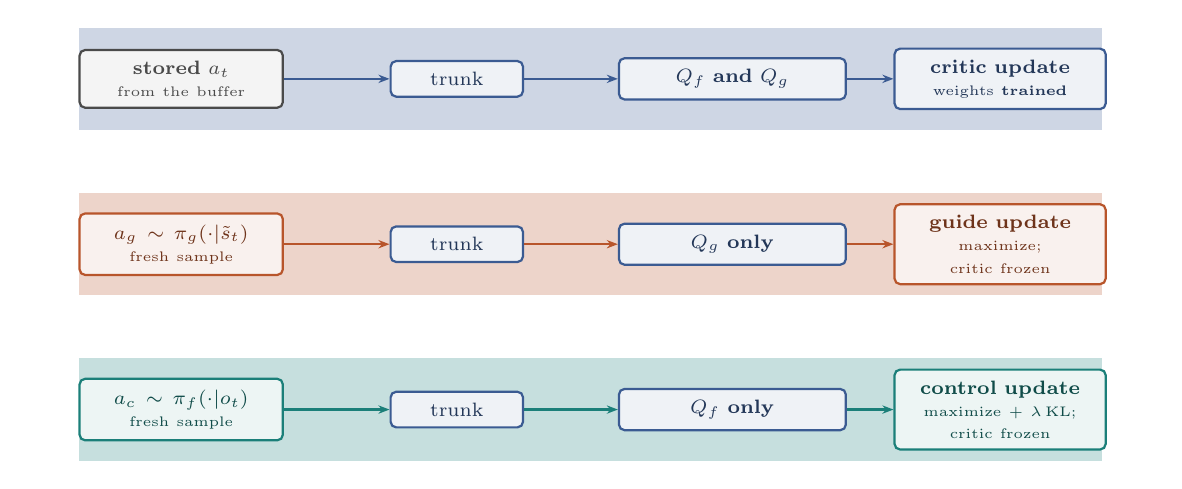
\begin{tikzpicture}[x=1cm, y=1cm]
    \foreach \y/\c in {2.1/cCritic, 0/cGuide, -2.1/cStudent}
      \draw[\c!25, line width=13mm] (-0.4,\y) -- (12.6,\y);

    % lane 1 — critic update
    \node[envb,   text width=2.3cm] (b1) at (0.9,2.1)  {\textbf{stored} $a_t$\\ \tiny from the buffer};
    \node[critic, text width=1.4cm] (t1) at (4.4,2.1)  {trunk};
    \node[critic, text width=2.6cm] (h1) at (7.9,2.1)  {$Q_f$ \textbf{and} $Q_g$};
    \node[critic, text width=2.4cm] (r1) at (11.3,2.1) {\textbf{critic update}\\ \tiny weights \textbf{trained}};
    \draw[arc] (b1) -- (t1); \draw[arc] (t1) -- (h1); \draw[arc] (h1) -- (r1);

    % lane 2 — guide actor update
    \node[guide, text width=2.3cm] (b2) at (0.9,0)  {$a_g \sim \pg(\cdot|\st)$\\ \tiny fresh sample};
    \node[critic, text width=1.4cm] (t2) at (4.4,0) {trunk};
    \node[critic, text width=2.6cm] (h2) at (7.9,0) {$Q_g$ \textbf{only}};
    \node[guide, text width=2.4cm] (r2) at (11.3,0) {\textbf{guide update}\\ \tiny maximize; critic frozen};
    \draw[arg] (b2) -- (t2); \draw[arg] (t2) -- (h2); \draw[arg] (h2) -- (r2);

    % lane 3 — control actor update
    \node[student, text width=2.3cm] (b3) at (0.9,-2.1)  {$a_c \sim \pf(\cdot|\ot)$\\ \tiny fresh sample};
    \node[critic,  text width=1.4cm] (t3) at (4.4,-2.1)  {trunk};
    \node[critic,  text width=2.6cm] (h3) at (7.9,-2.1)  {$Q_f$ \textbf{only}};
    \node[student, text width=2.4cm] (r3) at (11.3,-2.1) {\textbf{control update}\\ \tiny maximize $+\ \lambda\,$KL; critic frozen};
    \draw[ars] (b3) -- (t3); \draw[ars] (t3) -- (h3); \draw[ars] (h3) -- (r3);
  \end{tikzpicture}}
  \end{center}
  \vspace{0.2em}
  {\footnotesize The trunk is the \emph{same} network in all three lanes. Two rules make the
  whole design readable: the critic is \textbf{only ever trained on actions that were actually
  executed}, and each actor \textbf{only ever reads its own head-pair} --- so the student
  optimizes the value of the deployed policy and never the teacher's.}
\end{frame}

\begin{frame}{Why the guide needs its own value head}
  \begin{columns}[T]
    \begin{column}{0.47\textwidth}
      \begin{center}
        {\footnotesize \textbf{One critic (naive)}}\\[4pt]
        \scalebox{0.8}{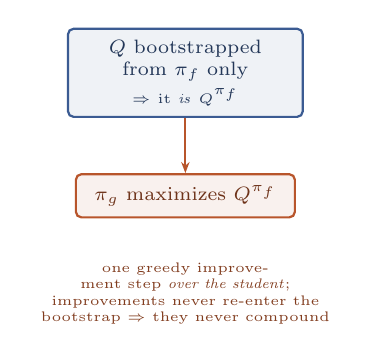
\begin{tikzpicture}
          \node[critic, text width=2.7cm] (q) at (0,0)
            {$Q$ bootstrapped from $\pf$ only\\[2pt] \tiny $\Rightarrow$ it \emph{is} $Q^{\pf}$};
          \node[guide, text width=2.5cm, below=7mm of q] (g) {$\pg$ maximizes $Q^{\pf}$};
          \draw[arg] (q) -- (g);
          \node[lbl, below=5mm of g, text width=3.9cm, align=center, text=cGuide!70!black]
            {one greedy improvement step \emph{over the student};\\ improvements never re-enter
             the bootstrap $\Rightarrow$ they never compound};
        \end{tikzpicture}}
      \end{center}
      \vspace{0.2em}
      {\scriptsize The teacher's advantage is
       \textcolor{cGuide!70!black}{\textbf{capped by construction}} --- contradicting the
       premise that a fully-observed teacher is meaningfully better.\par}
    \end{column}
    \begin{column}{0.47\textwidth}
      \begin{center}
        {\footnotesize \textbf{Two head-pairs (ours)}}\\[4pt]
        \scalebox{0.8}{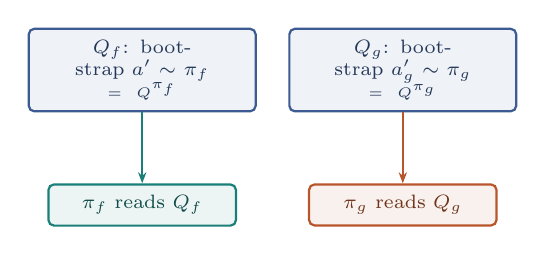
\begin{tikzpicture}
          \node[critic, text width=2.6cm] (qf) at (0,0)
            {$Q_f$: bootstrap $a' \!\sim\! \pf$\\ \tiny $= Q^{\pf}$};
          \node[critic, text width=2.6cm, right=4mm of qf] (qg)
            {$Q_g$: bootstrap $a_g' \!\sim\! \pg$\\ \tiny $= Q^{\pg}$};
          \node[student, text width=2.1cm, below=9mm of qf] (sf) {$\pf$ reads $Q_f$};
          \node[guide,   text width=2.1cm, below=9mm of qg] (sg) {$\pg$ reads $Q_g$};
          \draw[ars] (qf) -- (sf);
          \draw[arg] (qg) -- (sg);
        \end{tikzpicture}}
      \end{center}
      \vspace{0.2em}
      {\scriptsize Each actor optimizes against \emph{its own} fixed point, so the teacher can
       run ahead. The student still optimizes $Q^{\pf}$ --- the \textbf{deployed} policy's
       value.\par}
    \end{column}
  \end{columns}
  \vspace{0.5em}
  \begin{center}
    {\scriptsize This recovers, in twin-$Q$ form, the role of Çerçi's separate $V$ network.}
  \end{center}
\end{frame}

% =====================================================================
\section{Objectives}

\begin{frame}{Critic: one template, two instantiations}
  Both head-pairs are trained on the \textbf{same stored transition} $(\st, a_t, r, \tilde{s}_{t+n})$
  and differ only in the policy used to bootstrap:
  \[ y_\bullet \;=\; r^{(n)}_t \;+\; \gamma^{n}\Big(z - \alpha_\bullet \log \pi_\bullet(a'_\bullet \,|\, \cdot)\Big)(1-d) \]
  \begin{center}\footnotesize
  \begin{tabular}{lllc}
    \toprule
    \textbf{head-pair} & \textbf{bootstrap action} & \textbf{temperature} & \textbf{estimates} \\
    \midrule
    $Q_f$ & $a' \sim \pf(\cdot\,|\,o_{t+n})$ & $\alpha_f$ & $Q^{\pf}$ --- the deployed policy \\
    $Q_g$ & $a'_g \sim \pg(\cdot\,|\,\tilde{s}_{t+n})$ & $\alpha_g$ & $Q^{\pg}$ --- the teacher \\
    \bottomrule
  \end{tabular}
  \end{center}
  \[ \mathcal{L}_Q \;=\; \mathrm{CE}\big(\Pi[y_f]\,\big\|\,Q_{f,i}(\st,a_t)\big)
                       \;+\; \mathrm{CE}\big(\Pi[y_g]\,\big\|\,Q_{g,i}(\st,a_t)\big), \qquad i \in \{1,2\} \]
  {\footnotesize The critic is distributional: $z$ are fixed bin values and $\Pi$ projects the
  target back onto that support. $n$-step returns and the EMA target network come from the
  backbone unchanged.}
\end{frame}

\begin{frame}{Actors: one new term in the whole method}
  \textbf{Guide} --- ordinary SAC on privileged input, against its own heads:
  \[ \mathcal{L}_{\pg} \;=\; \mathbb{E}\Big[\, \alpha_g \log \pg(a_g|\st) \;-\; \min_i Q_{g,i}(\st, a_g) \,\Big] \]

  \textbf{Control} --- the same objective on proprioception, plus guidance:
  \[ \mathcal{L}_{\pf} \;=\; \mathbb{E}\Big[\, \alpha_f \log \pf(a_c|\ot) \;-\; \min_i Q_{f,i}(\st, a_c)
     \;+\; \underbrace{\lambda(t)\,\bar{q}\; D_{\mathrm{KL}}\big(\pf(\cdot|\ot)\,\big\|\,\mathrm{sg}[\pg(\cdot|\st)]\big)}_{\text{the only term Guided SAC adds}} \Big] \]

  \begin{itemize}\footnotesize
    \item \textbf{KL, not $L_2$.} Both policies are $\tanh$-Gaussian, so the KL is closed-form
          and matches the teacher's \emph{variance}, not just its mean --- the student may stay
          uncertain where the teacher is. The teacher is stop-gradded.
    \item $\bar{q} = \mathbb{E}|\min_i Q_{f,i}|$ keeps $\lambda$ dimensionless as values grow;
          $\alpha_f, \alpha_g$ are learned \textbf{separately}.
  \end{itemize}
\end{frame}

% =====================================================================
\section{Schedules}

\begin{frame}{Guidance is scheduled, grounding is not}
  \begin{center}
  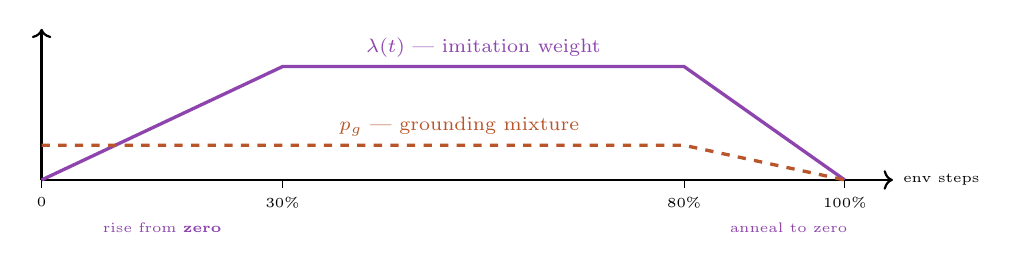
\begin{tikzpicture}[xscale=1.02, yscale=0.8]
    \draw[->, thick] (0,0) -- (10.6,0) node[right, font=\tiny] {env steps};
    \draw[->, thick] (0,0) -- (0,2.4);
    % lambda trapezoid
    \draw[very thick, cAccent] (0,0) -- (3,1.8) -- (8,1.8) -- (10,0);
    \node[font=\scriptsize, text=cAccent] at (5.5,2.1) {$\lambda(t)$ --- imitation weight};
    % p_g
    \draw[very thick, cGuide, dashed] (0,0.55) -- (8,0.55) -- (10,0);
    \node[font=\scriptsize, text=cGuide] at (5.2,0.85) {$p_g$ --- grounding mixture};
    % ticks
    \foreach \x/\l in {0/0, 3/30\%, 8/80\%, 10/100\%}
      \draw (\x,0) -- (\x,-0.12) node[below, font=\tiny] {\l};
    \node[font=\tiny, align=center, text=cAccent] at (1.5,-0.75) {rise from \textbf{zero}};
    \node[font=\tiny, align=center, text=cAccent] at (9.3,-0.75) {anneal to zero};
  \end{tikzpicture}
  \end{center}
  \begin{columns}[T]
    \begin{column}{0.5\textwidth}
      {\footnotesize \textbf{$\lambda$ starts at 0} because an unconverged teacher emits
      noise --- a constant weight injects it exactly when the student is most malleable.}
    \end{column}
    \begin{column}{0.5\textwidth}
      {\footnotesize \textbf{$\lambda$ ends at 0} so the student finishes under its own
      constraints --- the cheapest mitigation of the imitation gap.}
    \end{column}
  \end{columns}
  \vspace{0.2em}
  {\footnotesize \textbf{$p_g$ is on from step 0} --- not exploration but \emph{value grounding}:
  without the guide ever acting, $(\st,a_g)$ never enters the buffer and $Q_g$ is queried off
  its own training distribution.}
\end{frame}

\begin{frame}{The imitation gap --- the method's real weakness}
  $\pg$ solves the \emph{fully observed} MDP. $\pf$ must solve the \emph{POMDP}. These are
  different problems, and projecting one onto the other is not optimal in general.

  \vspace{0.5em}
  \begin{alertblock}{Concretely, for blind locomotion}
    A teacher that sees the height scan never learns to probe the ground with a foot, never
    steps cautiously into the unknown, never moves to enrich its own IMU signal --- it has no
    need to. Imitating it can therefore \emph{suppress exactly the behaviours that keep a
    blind robot alive}.
  \end{alertblock}

  \vspace{0.2em}
  {\footnotesize Mitigations built in, weakest to strongest:}
  \begin{enumerate}\footnotesize
    \item \textbf{KL rather than $L_2$} --- the student may stay uncertain where the teacher is.
    \item \textbf{$\lambda \to 0$} --- guidance is removed before training ends.
    \item \textbf{Latent supervision} (planned): supervise a learned \emph{representation}
          $\hat{z} = E(\ot)$ against privileged $z$ and let the policy decide how to use it ---
          closes the gap by construction.
  \end{enumerate}
\end{frame}

% =====================================================================
\section{Data flow}

\begin{frame}{Training loop}
  \begin{center}
  \scalebox{0.85}{%
  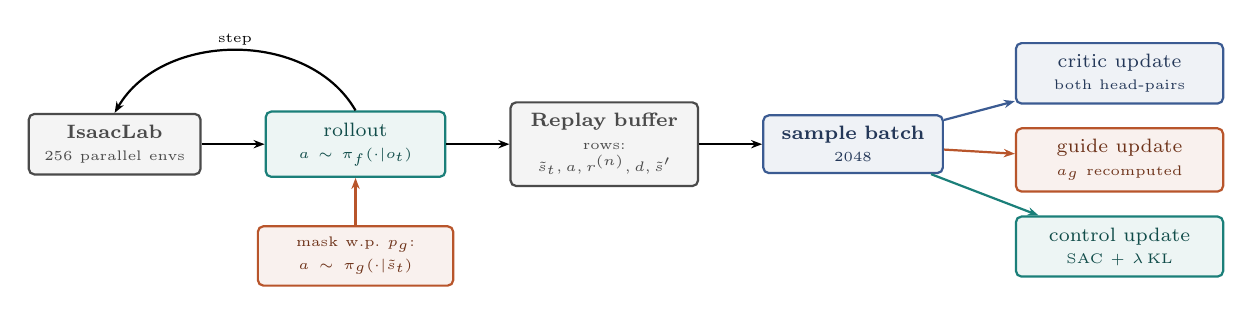
\begin{tikzpicture}[node distance=4mm]
    \node[envb, text width=1.9cm] (env) {\textbf{IsaacLab}\\ \tiny 256 parallel envs};
    \node[student, right=8mm of env, text width=2.0cm] (roll)
      {rollout\\ \tiny $a \sim \pf(\cdot|\ot)$};
    \node[guide, below=6mm of roll, text width=2.2cm] (mix)
      {\tiny mask w.p.\ $p_g$:\\ \tiny $a \sim \pg(\cdot|\st)$};
    \node[envb, right=8mm of roll, text width=2.1cm] (buf)
      {\textbf{Replay buffer}\\ \tiny rows: $\st,a,r^{(n)},d,\tilde{s}'$};
    \node[critic, right=8mm of buf, text width=2.0cm] (upd)
      {\textbf{sample batch}\\ \tiny 2048};

    \node[critic, right=9mm of upd, text width=2.35cm, yshift=9mm] (uc)
      {critic update\\ \tiny both head-pairs};
    \node[guide, right=9mm of upd, text width=2.35cm, yshift=-2mm] (ug)
      {guide update\\ \tiny $a_g$ recomputed};
    \node[student, right=9mm of upd, text width=2.35cm, yshift=-13mm] (us)
      {control update\\ \tiny SAC $+\ \lambda\,\mathrm{KL}$};

    \draw[ar] (env) -- (roll);
    \draw[arg] (mix) -- (roll);
    \draw[ar] (roll) -- (buf);
    \draw[ar] (buf) -- (upd);
    \draw[arc] (upd) -- (uc);
    \draw[arg] (upd) -- (ug);
    \draw[ars] (upd) -- (us);
    \draw[ar] (roll.north) to[out=120,in=60] node[lbl,above] {step} (env.north);
  \end{tikzpicture}}
  \end{center}
  \vspace{0.2em}
  \begin{itemize}\footnotesize
    \item $a_g$ is \textbf{never stored}. It is recomputed from the sampled batch's own
          $\st$ at update time, so teacher--state alignment is true by construction and the
          buffer schema is unchanged --- no off-by-one is even representable.
    \item Mixed rows are stored \textbf{unmarked}: off-policy TD does not need provenance.
  \end{itemize}
\end{frame}

\begin{frame}{Deployment --- what survives}
  \begin{center}
  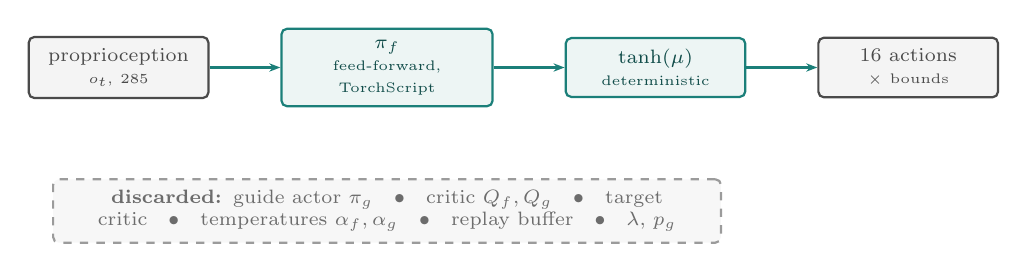
\begin{tikzpicture}[node distance=6mm]
    \node[envb, text width=2.0cm] (s) {proprioception\\ \tiny $\ot$, 285};
    \node[student, right=9mm of s, text width=2.4cm] (a) {$\pf$\\ \tiny feed-forward, TorchScript};
    \node[student, right=9mm of a, text width=2.0cm] (t) {$\tanh(\mu)$\\ \tiny deterministic};
    \node[envb, right=9mm of t, text width=2.0cm] (o) {16 actions\\ \tiny $\times$ bounds};
    \draw[ars] (s) -- (a); \draw[ars] (a) -- (t); \draw[ars] (t) -- (o);

    \node[dropb, below=9mm of a, text width=8.2cm]
      {\textbf{discarded:} guide actor $\pg$ \; $\bullet$ \; critic $Q_f,Q_g$ \; $\bullet$ \; target critic \;
       $\bullet$ \; temperatures $\alpha_f,\alpha_g$ \; $\bullet$ \; replay buffer \; $\bullet$ \; $\lambda$, $p_g$};
  \end{tikzpicture}
  \end{center}
  \vspace{0.4em}
  \begin{itemize}\footnotesize
    \item The deployed artifact is \textbf{architecturally identical} to a vanilla SAC actor.
          Guided training costs \emph{nothing} at inference --- the strongest practical
          argument for asymmetric methods.
    \item Nothing privileged can leak: the actor consumes a fixed 285-dim slice and the
          export path never reads the guide's files.
  \end{itemize}
\end{frame}

% =====================================================================
\section{Implementation}

\begin{frame}{Code map}
  Built as an \textbf{extension} of the FlashSAC backbone, never a fork: the vendored
  learning core is byte-identical, and without the \texttt{-{}-guided} flag the pipeline is
  the unmodified baseline.

  \vspace{0.5em}
  \begin{center}\footnotesize
  \begin{tabular}{ll}
    \toprule
    \texttt{gsac/config.py} & config dataclass; $\lambda(t)$, $p_g(t)$; fail-fast validation \\
    \texttt{gsac/network.py} & \texttt{GuidedDoubleCritic}: shared trunks $+$ second head-pair \\
    \texttt{gsac/update.py} & the three losses above, each traced to its source equation \\
    \texttt{gsac/agent.py} & \texttt{GuidedFlashSACAgent}: networks, rollout mixing, updates \\
    \midrule
    \texttt{train.py -{}-guided} & launcher flag; everything guided is behind it \\
    \bottomrule
  \end{tabular}
  \end{center}

  \vspace{0.6em}
  {\footnotesize The subclass overrides \texttt{sample\_actions}
  (mixing), \texttt{update} (the three losses) and \texttt{save}/\texttt{load} (guide checkpoints); everything else is inherited.}
\end{frame}

\begin{frame}{One codebase, four experiments}
  The mechanism decomposition is expressible as \emph{configuration}, which is what makes an
  honest ablation cheap:

  \vspace{0.5em}
  \begin{center}\footnotesize
  \begin{tabular}{llll}
    \toprule
    \textbf{Rung} & \textbf{Isolates} & \textbf{Setting} & \textbf{Cost} \\
    \midrule
    A1 & vanilla SAC & symmetric critic (override) & baseline \\
    A2 & \textbf{M1} asymmetric critic & \texttt{-{}-no-train\_guide} & no guide built \\
    A4 & \textbf{M2} grounding mixture & \texttt{-{}-lambda\_max 0} & guide trained, no imitation \\
    A5 & \textbf{M3} full Guided SAC & default & everything on \\
    \bottomrule
  \end{tabular}
  \end{center}

  \vspace{0.7em}
  \begin{block}{The question this design exists to answer}
    Which of the three mechanisms actually pays --- and is the second actor worth its cost?
    The literature has never separated them. Whatever the answer, it is informative.
  \end{block}
\end{frame}

\begin{frame}{Summary}
  \begin{itemize}
    \item Blind locomotion is a genuine POMDP; the simulator knows far more than the robot
          ever will.
    \item Guided SAC bundles three separable mechanisms. We keep the free one (asymmetric
          critic), soften the risky one (imitation via scheduled KL), and use the expensive
          one sparingly and for a different reason than the original (value grounding).
    \item The single-agent reduction is not a copy: the teacher needs \textbf{its own value
          head}, otherwise its advantage is capped by construction.
    \item The imitation gap is the method's real theoretical weakness; latent supervision is
          the principled successor if action-space imitation does not pay.
    \item \textbf{Deployment cost is exactly zero} --- the shipped network is a plain SAC actor
          on proprioception.
  \end{itemize}
\end{frame}

\end{document}
